\documentclass{article}
\usepackage{ifluatex}
\ifluatex 
    \usepackage{fontspec}
    \setsansfont[
        Path = C:/Windows/Fonts/,
        Extension = .ttf ,
        BoldFont={cmunsx} ,
        ItalicFont={cmunsi} ,
        BoldItalicFont={cmunso} ,
        UprightFont={cmunss}
    ]{CMU Sans Serif}
    \setmainfont[
        Path = C:/Windows/Fonts/,
        Extension = .ttf ,
        BoldItalicFont={cmunbi} ,
        ItalicFont={cmunti} ,
        BoldFont={cmunbx} ,
        UprightFont={cmunrm}
    ]{CMU Serif}
    \setmonofont[
        Path = C:/Windows/Fonts/,
        Extension = .ttf ,
        % LightFont={cmunbtl} ,
        BoldItalicFont={cmuntx} ,
        % LightItalicFont={cmunbto} ,
        BoldFont={cmuntb} ,
        ItalicFont={cmunit} ,
        UprightFont={cmuntt}
    ]{CMU Typewriter Text}
    \defaultfontfeatures{Ligatures={TeX}}
\else
    \usepackage[T2A]{fontenc}
    \usepackage[utf8]{inputenc}
\fi
\usepackage[english,russian]{babel}
\usepackage{anyfontsize}
\usepackage{amssymb,latexsym,amsmath,amscd,mathtools,wasysym,stmaryrd}
\usepackage[shortlabels]{enumitem}
\usepackage[makeroom]{cancel}
\usepackage{graphicx}
\usepackage{geometry}
\usepackage{verbatim}
\usepackage{fvextra}

\usepackage{longtable}
\usepackage{multirow}
\usepackage{multicol}
\usepackage{tabu}
\usepackage{arydshln} % \hdashline and :
\usepackage{makecell} % \makecell for line breaks
\usepackage{tabularx}
\usepackage{xltabular}
\renewcommand\tabularxcolumn[1]{m{#1}} % for vertical centering text in X column


\usepackage{float}
\makeatletter
\g@addto@macro\@floatboxreset\centering
\makeatother
\setlength{\parindent}{0pt}
\usepackage{caption}
\usepackage{csquotes}
\usepackage[bb=dsserif]{mathalpha}
\usepackage[normalem]{ulem}

\usepackage[e]{esvect}
\let\vec\vv

\usepackage[x11names]{xcolor}
\colorlet{darkgreen}{black!25!blue!50!green}


%% Here f*cking with mathabx
\DeclareFontFamily{U}{matha}{\hyphenchar\font45}
\DeclareFontShape{U}{matha}{m}{n}{
    <5> <6> <7> <8> <9> <10> gen * matha
    <10.95> matha10 <12> <14.4> <17.28> <20.74> <24.88> matha12
}{}
\DeclareSymbolFont{matha}{U}{matha}{m}{n}
\DeclareFontFamily{U}{mathb}{\hyphenchar\font45}
\DeclareFontShape{U}{mathb}{m}{n}{
    <5> <6> <7> <8> <9> <10> gen * mathb
    <10.95> matha10 <12> <14.4> <17.28> <20.74> <24.88> mathb12
}{}
\DeclareSymbolFont{mathb}{U}{mathb}{m}{n}

\DeclareMathSymbol{\tmp}{\mathrel}{mathb}{"15}
\let\defeq\tmp
\DeclareMathSymbol{\tmp}{\mathrel}{mathb}{"16}
\let\eqdef\tmp

\usepackage{trimclip}
\DeclareMathOperator{\updownarrows}{\clipbox{0pt 0pt 4.175pt 0pt}{$\upuparrows$}\hspace{-.825px}\clipbox{0pt 0pt 4.175pt 0pt}{$\downdownarrows$}}
\DeclareMathOperator{\downuparrows}{\clipbox{0pt 0pt 4.175pt 0pt}{$\downdownarrows$}\hspace{-.825px}\clipbox{0pt 0pt 4.175pt 0pt}{$\upuparrows$}}

\makeatletter
\providecommand*\deletecounter[1]{%
    \expandafter\let\csname c@#1\endcsname\@undefined}
\makeatother


\usepackage{hyperref}
\hypersetup{
    %hidelinks,
    colorlinks=true,
    linkcolor=darkgreen,
    urlcolor=blue,
    breaklinks=true,
}

\usepackage{pgf}
\usepackage{pgfplots}
\pgfplotsset{compat=newest}
\usepackage{tikz,tikz-3dplot}
\usepackage{tkz-euclide}
\usetikzlibrary{calc,automata,patterns,angles,quotes,backgrounds,shapes.geometric,trees,positioning,decorations.pathreplacing}
\usetikzlibrary{lindenmayersystems}
\pgfkeys{/pgf/plot/gnuplot call={cd Output && gnuplot}}
\usepgfplotslibrary{fillbetween,polar}
\usetikzlibrary{quotes,babel}
\ifluatex
\usetikzlibrary{graphs,graphs.standard,graphdrawing}
\usegdlibrary{layered,trees,circular,force}
\else
% \errmessage{Run with LuaTeX, if you want to use gdlibraries}
\fi
\makeatletter
\newcommand\currentnode{\the\tikz@lastxsaved,\the\tikz@lastysaved}
\makeatother

%\usepgfplotslibrary{external} 
%\tikzexternalize

\makeatletter
\newcommand*\circled[2][1.0]{\tikz[baseline=(char.base)]{
        \node[shape=circle, draw, inner sep=2pt,
        minimum height={\f@size*#1},] (char) {#2};}}
\makeatother

\newcommand{\existence}{{\circled{$\exists$}}}
\newcommand{\uniqueness}{{\circled{$\hspace{0.5px}!$}}}
\newcommand{\rightimp}{{\circled{$\Rightarrow$}}}
\newcommand{\leftimp}{{\circled{$\Leftarrow$}}}

\DeclareMathOperator{\sign}{sign}
\DeclareMathOperator{\Cl}{Cl}
\DeclareMathOperator{\proj}{pr}
\DeclareMathOperator{\Arg}{Arg}
\DeclareMathOperator{\supp}{supp}
\DeclareMathOperator{\diag}{diag}
\DeclareMathOperator{\tr}{tr}
\DeclareMathOperator{\rank}{rank}
\DeclareMathOperator{\Lat}{Lat}
\DeclareMathOperator{\Lin}{Lin}
\DeclareMathOperator{\Ln}{Ln}
\DeclareMathOperator{\Orbit}{Orbit}
\DeclareMathOperator{\St}{St}
\DeclareMathOperator{\Seq}{Seq}
\DeclareMathOperator{\PSet}{PSet}
\DeclareMathOperator{\MSet}{MSet}
\DeclareMathOperator{\Cyc}{Cyc}
\DeclareMathOperator{\Hom}{Hom}
\DeclareMathOperator{\End}{End}
\DeclareMathOperator{\Aut}{Aut}
\DeclareMathOperator{\Ker}{Ker}
\DeclareMathOperator{\Def}{def}
\DeclareMathOperator{\Alt}{Alt}
\DeclareMathOperator{\Sim}{Sim}
\DeclareMathOperator{\Int}{Int}
\DeclareMathOperator{\grad}{grad}
\DeclareMathOperator{\sech}{sech}
\DeclareMathOperator{\csch}{csch}
\DeclareMathOperator{\asin}{\sin^{-1}}
\DeclareMathOperator{\acos}{\cos^{-1}}
\DeclareMathOperator{\atan}{\tan^{-1}}
\DeclareMathOperator{\acot}{\cot^{-1}}
\DeclareMathOperator{\asec}{\sec^{-1}}
\DeclareMathOperator{\acsc}{\csc^{-1}}
\DeclareMathOperator{\asinh}{\sinh^{-1}}
\DeclareMathOperator{\acosh}{\cosh^{-1}}
\DeclareMathOperator{\atanh}{\tanh^{-1}}
\DeclareMathOperator{\acoth}{\coth^{-1}}
\DeclareMathOperator{\asech}{\sech^{-1}}
\DeclareMathOperator{\acsch}{\csch^{-1}}

\newcommand*{\scriptA}{{\mathcal{A}}}
\newcommand*{\scriptB}{{\mathcal{B}}}
\newcommand*{\scriptC}{{\mathcal{C}}}
\newcommand*{\scriptD}{{\mathcal{D}}}
\newcommand*{\scriptF}{{\mathcal{F}}}
\newcommand*{\scriptG}{{\mathcal{G}}}
\newcommand*{\scriptH}{{\mathcal{H}}}
\newcommand*{\scriptK}{{\mathcal{K}}}
\newcommand*{\scriptL}{{\mathcal{L}}}
\newcommand*{\scriptM}{{\mathcal{M}}}
\newcommand*{\scriptP}{{\mathcal{P}}}
\newcommand*{\scriptQ}{{\mathcal{Q}}}
\newcommand*{\scriptR}{{\mathcal{R}}}
\newcommand*{\scriptT}{{\mathcal{T}}}
\newcommand*{\scriptU}{{\mathcal{U}}}
\newcommand*{\scriptX}{{\mathcal{X}}}
\newcommand*{\Cnk}[2]{\left(\begin{matrix}#1\\#2\end{matrix}\right)}
\newcommand*{\im}{{\mathbf i}}
\newcommand*{\id}{{\mathrm{id}}}
\newcommand*{\compl}{^\complement}
\newcommand*{\dotprod}[2]{{\left\langle{#1},{#2}\right\rangle}}
\newcommand\matr[1]{\left(\begin{matrix}#1\end{matrix}\right)}
\newcommand\matrd[1]{\left|\begin{matrix}#1\end{matrix}\right|}
\newcommand\arr[2]{\left(\begin{array}{#1}#2\end{array}\right)}

\DeclareMathOperator{\divby}{\scalebox{1}[.65]{\vdots}}
\DeclareMathOperator{\toto}{\rightrightarrows}
\DeclareMathOperator{\ntoto}{\not\rightrightarrows}

\newcommand{\bigmid}{\mathrel{\big|}}
\newcommand{\Bigmid}{\mathrel{\Big|}}
\newcommand{\biggmid}{\mathrel{\bigg|}}

\newcommand{\undercolorblack}[2]{{\color{#1}\underline{\color{black}#2}}}
\newcommand{\undercolor}[2]{{\colorlet{tmp}{.}\color{#1}\underline{\color{tmp}#2}}}

\usepackage{adjustbox}

\geometry{margin=1in}
\usepackage{fancyhdr}
\pagestyle{fancy}
\fancyfoot[L]{}
\fancyfoot[C]{Иванов Тимофей}
\fancyfoot[R]{\pagename\ \thepage}
\fancyhead[L]{}
\fancyhead[R]{\leftmark}
\renewcommand{\sectionmark}[1]{\markboth{#1}{}}

\setcounter{tocdepth}{5}
\usepackage{amsthm}
\usepackage{chngcntr}

\theoremstyle{definition}
\newtheorem{definition}{Определение}
\counterwithin*{definition}{section}

\theoremstyle{plain}
\newtheorem{theorem}{Теорема}
\counterwithin*{theorem}{section} % Without changing appearance
\newtheorem{lemma}{Лемма}
\counterwithin*{lemma}{section}
\newtheorem{corollary}{Следствие}[theorem]
\counterwithin{corollary}{theorem} % Changing appearance
\counterwithin{corollary}{lemma}
\newtheorem*{claim}{Утверждение}
\newtheorem{property}{Свойство}[definition]

\theoremstyle{remark}
\newtheorem*{remark}{Замечание}
\newtheorem*{example}{Пример}

\newtheorem*{discourse}{Рассуждение}


%\renewcommand\qedsymbol{$\blacksquare$}

\counterwithin{equation}{section}

\input{Headers/graphs}

\usepackage[outputdir=Output, cache=false]{minted}

\begin{document}
    \begin{itemize}
        \item Exploratory DA~--- анализ (чаще всего глазками) данных, чтобы найти в нём пропуски, выбросы и прочий мусор, который вы можете глазами найти. Тут же вы думаете о том, чем эти данные являются, и как их хранить. А ещё тут вы можете формировать базовые гипотезы.
        \item Confirmatory DA~--- не рассказали, что такое.
        \item Показательный анализ данных~--- машинное обучение с целью что-нибудь предсказывать.
        \item Визуализация данных.
    \end{itemize}
    Знание~--- закономерность в некоторой области, которые позволяют решать проблемы.\\
    Data Mining~--- один из этапов в извлечении знаний из данных. Тут три этапа:
    \begin{enumerate}
        \item Сбор данных.
        \item Выделение признаков.
        \item Применение ML.
    \end{enumerate}
    Фактически это как DA, но с акцентом на немного другое.\\
    Data Science:
    \begin{itemize}
        \item Сбор данных.
        \item Интеграция данных (data integration).
        \item Хранение данных (data warehousing).
        \item Анализ данных.
        \item Высокопроизводительные вычисления (high-performance computing).
    \end{itemize}
    Как это с точки зрения бизнеса выглядит? Есть CRISP-DM:
    \begin{enumerate}
        \item Понимание бизнеса (перевод слов заказчика на что-то понятное).
        \item Понимание данных (требование правильных данных от заказчика).
        \item Подготовка данных (понять, как хранить данные).
        \item Моделирование (собственно, решать задачу).
        \item Оценка (понять, что мы получили).
        \item Если всё хорошо, внедряем, заворачиваем в красивую обёртку и т.п.
    \end{enumerate}
    \paragraph{Данные.}
    Данные бывают структурированные, неструктурированные и частично структурированные. Чаще всего мы встречаем неструктурированные. Это видео, посты в соцсетях и любая другая хрень, которую мы встречаем. Частично структурированные~--- XML, JSON и прочий мусор, который до полностью структурированных не дотягивает. А полностью структурированные данные~--- это матрицы (из $n$ объектов по $m$ характеристик у каждого).\\
    Имея неструктурированные или частично структурированные данные, мы почти всегда хотим его структурировать, чтобы было удобнее.\\
    В DA строку матрицы называют object, instance, sample, example и как угодно ещё, а столбец матрицы~--- feature, attribute, characteristic или factor.\\
    Что важно про наши матрицы? Чтобы порядок столбцов и строк был не важен. Если ваш алгоритм не такой, это странно. Исключение: временной ряд.
    \paragraph{Признаки.}
    Глобально их два: категория и число (качество и количество). Первое дискретно, второе непрерывно, категории мы можем только на равенство проверять, а с числами можем арифметику делать. Категориям обычно целое число сопоставляют, чтобы удобно было. Но есть и другие типы, например, порядковый: дискретный, но есть порядок. Впрочем, очень часто он сводится к либо к категории, либо к числу.\\
    С числами работать гораздо удобнее, но если надо, легко можно дискретизировать наше число любом образом (например, баллы в оценку~--- дискретизация). Как преобразовать порядковый тип во что-то? Можно преобразовать в число через порядковый номер. А можно в категорию, создав $k$ бинарных значений вида ${}<x$.\\
    \subparagraph{One-hot encoding.}
    Берём категорию из $k$ значений, преобразуем в $k$ булевых категорий вида ${}=c_i$, а потом из истины сделать 1, а из лжи~--- 0. Отличный план, как из категории сделать число.\\
    Ещё можно преобразовывать иначе, например категории сопоставлять случайный вектор или число, бинарное представление которого используется как новые признаки.\\
    Важное примечание: числа~--- не всегда числа. Например, если мы цифры распознаём, то плохо считать числа числами, а не категориями. Потому что изображение тройки не находится между изображением двойки и четвёрки. Поэтому аккуратно с преобразованием категорий в числа.\\
    Ещё интересность: время. Если у нас есть периоды, то хреначим синус и косинус, чтобы периодично было:
    \[
    f_{2e-1}=\sin\frac{2\pi t}{T_e}\qquad\qquad f_{2e}=\cos\frac{2\pi t}{T_e}
    \]
    Или ещё интересность, цвет. Цвет кодируем в RGB, а не в HSV/HSB, потому что там тон цвета неоднозначный. Красный~--- это и 0, и 360.\\
    Как хранить данные? Самый простой формат: CSV. Он плохо стандартизирован, правда. А ещё его недостаток в том, что там шапки нет. Нет ни информации о типах, ничего. Если хочется более человеческого~--- ARFF: примерно как CSV, но более стандартизирован и имеет шапку с типами данных. Типы: Numeric (число), Nominal (категория), String и Date.
    \begin{figure}[H]
        \centering
        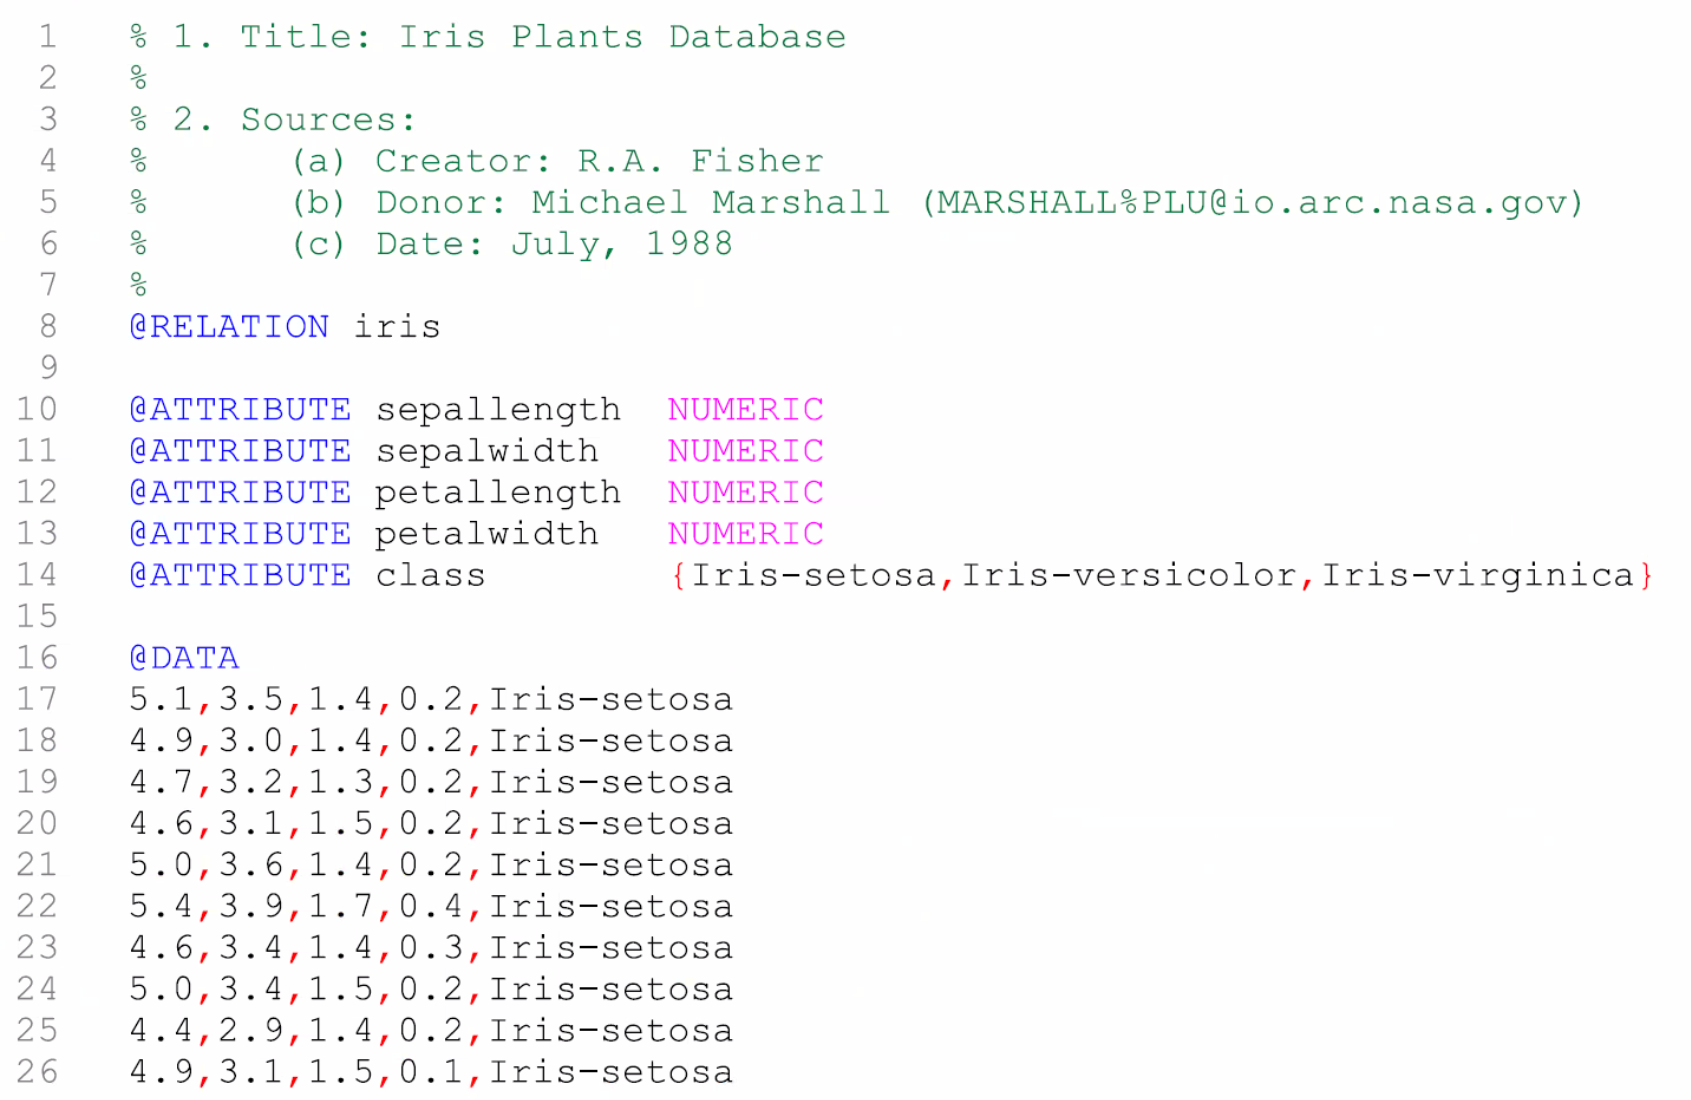
\includegraphics[width=0.9\linewidth]{Images/ARFF-example}
        \label{fig:arff-example}
    \end{figure}\noindent
    Прочие типы данных.
    \begin{itemize}
        \item Картинка. Самое простое~--- двух- (или трёх-)мерная матрица. И есть 1000 алгоритмов, как привести её в один вектор (притом довольно маленький).
        \item Текст. Тут сложнее. Самое тупое~--- посчитать частоту слов. Но не надо, тут сразу двигайте в сторону LLM.
        \item Звук. Это сигнал во времени, и самый простой вариант его представить~--- вектор значений. Для него тоже есть всякие штуки типа спектрограммы Мэла, чтобы преобразовывать звук во что-то более адекватное.
        \item Видео. Это мультимодальный объект, то есть объект, в котором разные типы внутри. Их анализировать тоже своими методами.
    \end{itemize}
    \paragraph{Нормализация.} Зачем? Чтобы признаки с большей дисперсией не влияли на результат сильнее остальных.\\
    Как? Сначала отбросим единицы измерения. Чтобы это было корректно, алгоритм должен быть инвариантен относительно линейных преобразований над признаками. А дальше надо как-то нормализовать дисперсию. Можно, например, вычесть из каждого признака минимум и поделить на разность между максимумом и минимумом. Это $[0;1]$-масштабирование. А ещё можно вычесть (выборное) мат. ожидание из признака и поделить на (выборное) стандартное отклонение это Z-масштабирование. Способов ещё куча, но это два простых.\\
    Как жить с ситуацией, когда у нас признаки зависимы? Никак не жить, если так, вы плохо собрали данные.
    \paragraph{Веса и сэмплирование.}
    Отлично, мы всё нормализовали, а теперь у нас из специфики задачи какие-то признаки более важны. Или могут быть объекты более важны.\\
    Говорят, что объект/признак обладает весом $w$, если он в $w$ раз больше влияет на результат. Если $w$ целое, то это эквивалентно тому, что объект/признак встречается $w$ раз.\\
    Примеры: учёт веса признака
    \[
    \operatorname{dist}(a;b)=\sqrt{\sum\limits_{j=1}^mw_j(a_j-b_j)^2}
    \]
    учёт веса объекта:
    \[
    \mathfrak L_D(\theta)=\sum\limits_{x\in D}w(x)\mathfrak L(x;\theta)
    \]
    А есть сэмплирование: вместо вхождения кучу раз в датасет мы можем сэмплировать объекты с вероятностью $\frac{w_j}{\sum w_j}$.\\
    Ещё это может использоваться для балансировки. Если вы знаете, что реальное распределение не очень сочетается с распределением данных, то мы можем пореже выбирать объекты мажоритарного класса или почаще объекты миноритарного класса (например, в данных одна группа большая, а другая~--- маленькая, а в жизни они равны, и мы даём большие веса малой группе). Да и в принципе, если нас не интересует распределение признаков по классам, распределение будет чаще подсовывать вам штуки из мажоритарного класса, что вам не всегда хочется.\\
    Как сэмплировать? Можно рандомно, можно каждый $x$-тый объект (систематически), можно стратифицированно (ровно в соотношение с какой-то категорией), можно кластерное (если кто-то уже за нас разбил объекты на множества, их множеств можно выбрать несколько).
    \paragraph{Шум.}
    Аномалии~--- плохие объекты для модели. Ошибки~--- плохие объекты для реальности. Пример: пусть у нас есть расход топлива автомобилями. И у нас у одного указан 30л / 100км. Если это грузовой автомобиль, а остальные~--- легковые, то это аномалия. А если объект всем хорош, и данные такие, то это ошибка (а возникнуть такое могло из-за того, что кто-то подразумевал мили на галлон).\\
    Пропуски в наборе данных. Откуда? Из склейки разных наборов данных, из изначально херовых данных или откуда угодно ещё. В CSV нет стандартного способа это обозначить, в ARFF это вопросик, а ещё можно специальное значения: None/Null для строк, категория с несуществующим номером для категорий или NaN для числа. Что делать с этим? Вырезать (признак или объект), заменить (заполнить пропуск средним арифметическим/модой/алгоритмом предсказания, который умеет в пропуски) или добавить (добавить новый признак, который говорит, были ли пропуск или нет; если там была категория, можно отдельное значение категории туда добавить, а не новое свойство делать).
\end{document}